%%%%%%%%%%%%%%%%%%%%%%%%%%%%%%%%
%%%%%   CLASSICAL MODELS   %%%%%
%%%%%%%%%%%%%%%%%%%%%%%%%%%%%%%%
\chapter[Analysis of prevalence of infection using generalised linear models]{Analysis of prevalence of infection using generalised linear models}
\label{ch:4.0}

% \textcolor{red}{RISK FACTORS aqui não faz muito sentido -- trocar por transmission determinants}
% \textcolor{red}{E tenho de chegar ao fim e dizer os transmission determinants são estes:...}
Prevalence of infection can be studied through the use of the generalised linear models (GLMs).
These models use the infection status of an individual as outcome of interest.
% \textcolor{red}{Isto está pouco perceptível, posso tirar: The use of this response variable can recreate the sensitivity of the most common malaria approaches when it comes to analyse transmission rate patterns across different defined regions.}
% \textcolor{red}{Não há necessidade: To explain the outcome, a combination of explanatory variables onto a GLMs' systematic component were used to reproduce the closest representation to the real life scenario as possible.}
The analysis of a GLM can help to explain how each covariate adds either an increase or decrease effect on the risk of infection.
Throughout this chapter, the significance level for all statistical hypothesis testing remained fixed at 0.05.
%Throughout the chapter, the use of the generalised linear models (GLMs) with different associated link functions allows for the understanding of the expected patters for prevalence of infection, as well as population-level transmission intensity.
%By developing and analysing different possible GLMs, one can then understand the effects, either harmful or protective, that each variable adds up to the prevalence of infection.
%characterising the status of each individual.
%This response variable is then set to be explained by different possible linear combinations of the remaining explanatory variables that define the systematic component.
%The model structure is linked by a link function, 

%The main objective in this chapter is to develop the best rational representation of the real life situation in which the data were collected.
%The first step is to create different demographical structures for the systematic component that would fit the prevalence model.
%These linear combinations of the explanatory variables are created based on theoretical relationships among them.


%%%%%%%%%%%%%%%%%%%%
% DATA PREPARATION %
%%%%%%%%%%%%%%%%%%%%
\section{Data preparation} \label{sec:4.1}

When using GLMs, the probability of an individual from a population being identified as infected depends on the values of multiple explanatory variables, i.e., the risk factors or transmission determinants.
Depending on the values when presented, the transmission determinants can influence the risk of infection, thus characterising the transmission heterogeneity recorded at different sites.
To compare how malaria transmission behaves across the different surveyed sites, the best approach was to identify a baseline village from which all results could be compared to.
The single village from West Usambara 3, Mgome, was the one selected.
With this village as reference, its altitude -- the lowest recorded -- was subtracted to the values from the explanatory variable \textit{Altitude}, allowing to interpret the null values of this quantitative variable.
Starting at Mgome (0 meters), each unit value incremented in the transmission determinant \textit{Altitude} represented a 100 meters high increase.


All explanatory variables here were categorical with the exception of \textit{Altitude}, being fitted into the models as factors with different levels.
To each factor was attributed a level corresponding to the baseline reference, from where the remaining levels were to be compared to.
The reference level from \textit{AgeGp} was the age group of individuals with ages within the interval of 1 to 4 years old, $\textit{Agegp}_{1-4}$.
Binary factor \textit{Gender} had its first level characterising a female individual and the second level a male one.
With Mgome as reference, the dominant ethnic group from the village, $\textit{EthGp}_{Other}$, was the indicator level from variable \textit{EthGp}, and West Usambara 3 ($\textit{Transect}_{WU3}$) the baseline factor from variable \textit{Transect}.
All three binary variables representing the antigens \textit{MSP1}, \textit{MSP2}, and \textit{AMA1}, had their reference levels corresponding to the absence of each respective antigen.

%%%%%%%%%%%%%%%%%%%%%%%%%%%%%%
% MODEL BUILDING & SELECTION %
%%%%%%%%%%%%%%%%%%%%%%%%%%%%%%
\section{Model fitting and selection}

When contemplating the potential transmission determinants in a model, their presence or absence may cause different impacts on the prevalence of malaria infection.
To study how influential these variables might be, simple univariate GLMs were fitted \cite{collet2003modelling}.
From an analysis of deviance, variables that more effectively could change the outcome results on their own were identified (Table \ref{tab:risk.factors}).
% it is possible to identify which exposure factors can more effectively change the outcome results on their own (Table \ref{tab:risk.factors}).
Determinants \textit{Transect} and \textit{Altitude} appeared as the more informative variables.
The logarithmic transformation of \textit{Altitude} was firstly thought as a way to reduce variability of the data, although it turned out causing a reduced change in deviance, being less impactful than the original continuous variable.
Further analysis under the logit link function showed a relationship between the response variable and \textit{Altitude}, thus being preferred to the use of the transformed variable (Figure \ref{fig:altitude_curve}).
% This transformed variable was rejected from further use.
%This transformation can still be used upon building the GLMs, although the non-transformed risk factor should be preferred.
\\

\begin{table}[h!]
\centering
\caption[Change in deviance for the studied univariate GLMs.]{Change in deviance for the variables considered for the prevalence of infection logistic GLMs (with respective degrees of freedom). P-values result from testing the significance of the model against the null model containing no explanatory variables. P-values $>0.05$ indicate the constructed univariate model is not statistically different than the null model.}
\label{tab:risk.factors}
\begin{tabular}{crr} 
\toprule
Risk factor   & \multicolumn{1}{c}{\begin{tabular}[c]{@{}c@{}}Change in\\deviance (d.f.)\end{tabular}} & p-value \\ 
\midrule
\textit{Altitude}      & 460.07 (1)   & $<0.001$  \\
log(\textit{Altitude}) & 437.54 (1)   & $<0.001$  \\
\textit{AgeGp}         & 76.62 (2)    & $<0.001$  \\
\textit{Gender}        & 3.13 (1)     & 0.0767    \\
\textit{EthGp}        & 379.56 (3)   & $<0.001$  \\
\textit{Transect}      & 482.73 (5)   & $<0.001$  \\
\textit{MSP1}          & 156.23 (1)   & $<0.001$  \\
\textit{MSP2}          & 223.58 (1)   & $<0.001$  \\
\textit{AMA1}          & 324.75 (1)   & $<0.001$  \\
\bottomrule
\end{tabular}
\end{table}

Only the univariate model containing the factor \textit{Gender}, with one degree of freedom, did not reject the null hypothesis for equality when compared to a null model without explanatory variables (p-value $>0.05$).
However, despite not being significant, and even though it caused the lesser impact on the deviance, \textit{Gender} was still considered for the models' construction.

\newpage

\begin{figure}[H]
\center
\begin{adjustbox}{width=14cm}
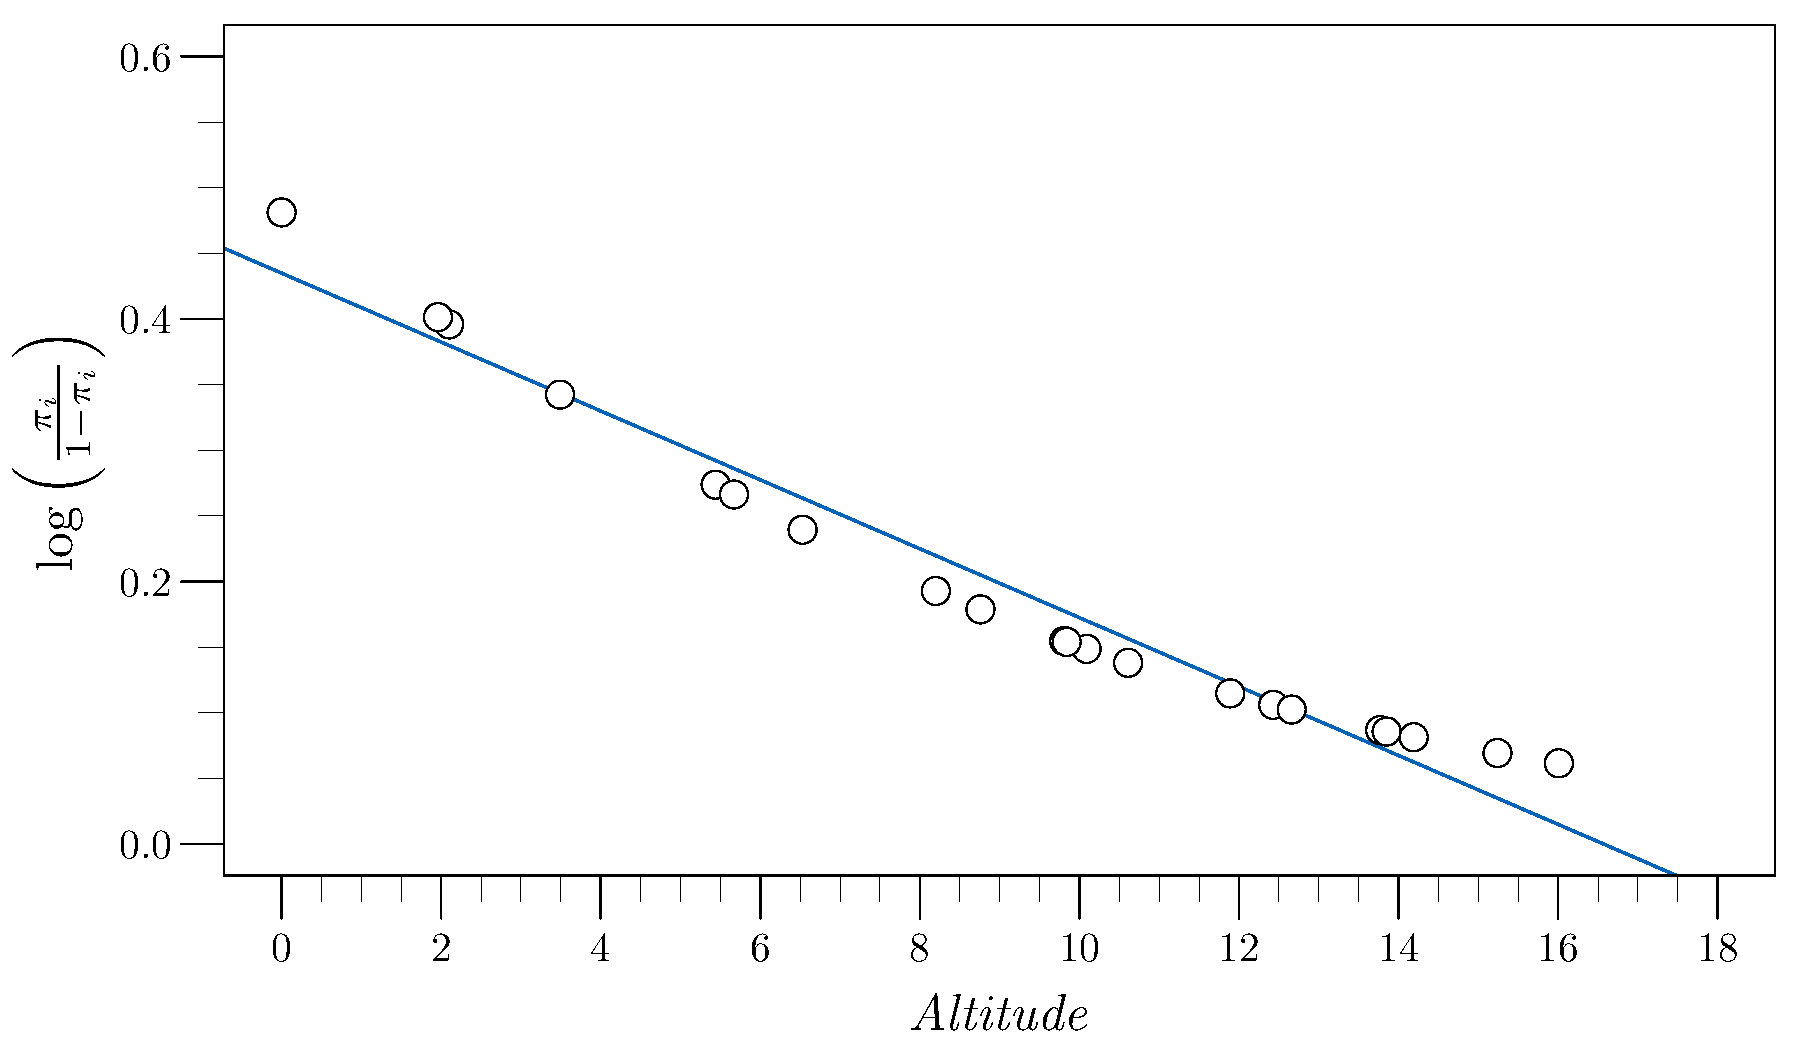
\includegraphics{images/altitude.pdf}
\end{adjustbox}
\caption[Relationship between transmission determinant \textit{Altitude} and respective log odds]{Relationship between prevalence of infection and the transmission determinant \textit{Altitude}. Starting at 0 meters, each unit in the \textit{Altitude} axis represents an increment in 100 meters high.}
\label{fig:altitude_curve}
\end{figure}

For inference purposes, the transmission determinants presented were separated into two different groups.
The first group encompassed the `demographical determinants', all variables characterising the environmental effects and individual characteristics that influenced the outcome.
Risk factors \textit{Transect}, \textit{Altitude}, \textit{AgeGp}, \textit{Gender}, and \textit{EthGp} belong in this group.
A second group identified the `exposure antigens', \textit{MSP1}, \textit{MSP2}, and \textit{AMA1}.
This approach allowed the creation of a first set of models and explain prevalence of infection based exclusively on demographical variables.
Afterwards, the more informative systematic structure was selected and used as reference when adding the exposure factors.
The addition of exposure antigens can be used to indicate the level of exposure to malaria parasites (Table \ref{tab:glm.formulas}).
%The antigens presented mostly work as markers for malaria exposure rather than conferring a noticeable immunological uplift \cite{}, the impact in prevalence reduction is not major.

\begin{table}[ht!]
\centering
\caption[Structure of systematic components used in the GLMs]{Structure of all GLMs' systematic components created, with respective degrees of freedom. Each model assumes probability of infection as response variable. Models \texttt{fit1} to \texttt{fit3} exclusively use variables from the demographical determinants. The following models add variables from the exposure antigens. The exposure transmission determinants are added in order, first individually (models \texttt{fit4} through \texttt{fit6}), and then pairing them up in two (\texttt{fit7}, \texttt{fit8}, and \texttt{fit9}). The last two models (\texttt{fit10} and \texttt{fit11}) add all three exposure factors to the \texttt{fit2} and \texttt{fit3} systematic structures.}
\label{tab:glm.formulas}
\begin{adjustbox}{width=\linewidth}
\begin{tabular}{llc} 
\toprule
Model   &  \multicolumn{1}{c}{Terms fitted in model}   &   d.f  \\
\midrule
\texttt{fit1}   & \textit{Altitude} + \textit{AgeGp} + \textit{Gender} + \textit{EthGp} + \textit{Transect}   & 5045   \\
\texttt{fit2}   & \textit{Altitude} $\times$ \textit{AgeGp} + \textit{Gender} + \textit{EthGp} + \textit{Transect}   & 5043   \\
\texttt{fit3}   & \textit{Altitude} $\times$ \textit{AgeGp} + \textit{Gender} + \textit{EthGp} $\times$ \textit{Transect}   & 5039   \\
\texttt{fit4}   & \textit{Altitude} $\times$ \textit{AgeGp} + \textit{Gender} + \textit{EthGp} + \textit{Transect} + \textit{MSP2}  & 5042   \\
\texttt{fit5}   & \textit{Altitude} $\times$ \textit{AgeGp} + \textit{Gender} + \textit{EthGp} + \textit{Transect} + \textit{MSP1}   & 5042   \\
\texttt{fit6}   & \textit{Altitude} $\times$ \textit{AgeGp} + \textit{Gender} + \textit{EthGp} + \textit{Transect} + \textit{AMA1}   & 5042   \\
\texttt{fit7}   & \textit{Altitude} $\times$ \textit{AgeGp} + \textit{Gender} + \textit{EthGp} + \textit{Transect} + \textit{MSP1} + \textit{MSP2}  & 5041   \\
\texttt{fit8}   & \textit{Altitude} $\times$ \textit{AgeGp} + \textit{Gender} + \textit{EthGp} + \textit{Transect} + \textit{MSP2} + \textit{AMA1}  & 5041   \\
\texttt{fit9}   & \textit{Altitude} $\times$ \textit{AgeGp} + \textit{Gender} + \textit{EthGp} + \textit{Transect} + \textit{MSP1} + \textit{AMA1}   & 5041   \\
\texttt{fit10}   & \textit{Altitude} $\times$ \textit{AgeGp} + \textit{Gender} + \textit{EthGp} + \textit{Transect} + \textit{MSP1} + \textit{MSP2} + \textit{AMA1}   & 5040   \\
\texttt{fit11}   & \textit{Altitude} $\times$ \textit{AgeGp} + \textit{Gender} + \textit{EthGp} $\times$ \textit{Transect} + \textit{MSP1} + \textit{MSP2} + \textit{AMA1}   & 5036   \\
\bottomrule
\end{tabular}
\end{adjustbox}
\end{table}

The first structure built, \texttt{fit1}, described malaria prevalence as a function of all demographical determinants with no interactions considered.
%Systematic component fit2 uses the logarithmic transformation of \textit{Altitude}.
%This transformation, firstly thought to help reducing the variability of the data, turned out less impactful than the original risk factor used in fit1, being discarded on the following models.
When recreating malaria prevalence over different time points, the age (or in this case the age group) of an individual is an important risk factor to consider, as it can be a categorical proxy for time of exposure.
%The constant exposure or recurrent infections to endemic malaria causes individuals to develop protective immunity and consequently reducing its prevalence rate at older age groups.
With \textit{Altitude} being a proxy for transmission intensity, the empirical association between this variable and \textit{AgeGp} (\texttt{fit2} and \texttt{fit3}) was expected to more accurately represent the altitude-dependent prevalence values.
% to recreate a peak-shift effect on the altitude-dependent prevalence values.
Under this interaction, the prevalence of infection should present higher values at age group 1$-$4, decreasing to lower estimates until the higher age group 15$-$45.
However, the maximum prevalence reached depends on the continuous \textit{Altitude}, as lower altitude sites have higher transmission intensities recorded.
With each transect mostly represented by a single ethnic group, the structure from \texttt{fit3} recreated the association between variables \textit{EthGp} and \textit{Transect}.

Afterwards, the addition of exposure variables onto the models was made gradually.
Starting at \texttt{fit4}, the exposure antigens were added to the previous model structure from \texttt{fit2}.
First, a single exposure transmission determinant was added to the model.
Factor \textit{MSP2} was added in \texttt{fit4}, \textit{MSP1} in \texttt{fit5}, and \textit{AMA1} was added in \texttt{fit6}.
The comparison of the three models should clarify for a better understanding of how sensitive the antigens are to the presence of infection (their immunogenicity).
%immunogenic they are (i.e. how quickly the antigens react upon exposure to malaria).
Using \texttt{fit2}'s demographical structure, models \texttt{fit7}, \texttt{fit8}, and \texttt{fit9}, added two exposure factors.
Systematic component from \texttt{fit7} included both \textit{MSP1} and \textit{MSP2}, fit8 incorporated \textit{MSP2} and \textit{AMA1}, and \texttt{fit9} built \textit{MSP1} and \textit{AMA1}.
These models functioned as an intermediary complement between the addition of a single antigen factor, and the inclusion of all three.
The order by which the exposure variables were included was based on previous knowledge that specific antigens MSP1 and AMA1 are more impactful than MSP2.
Finally, \texttt{fit10} included all exposure risk factors into \texttt{fit2}'s systematic structure.
The systematic component \texttt{fit11} then extended all three exposure antigens onto the demographical systematic structure from \texttt{fit3}, with a relation between \textit{EthGp} and \textit{Transect}.
%Models fit5 to fit11 are extensions of the peak-shift model fit3, with model fit12 deriving from the structure of the demographical model fit4.
%Models fit5, fit6, and fit7, add each antigen variable individually and can be used to compare the influence each one as on the information gained.
%Since all antigens presented mostly work as markers for malaria exposure rather than conferring a noticeable immunological uplift \cite{}, their impact in prevalence reduction should not be major.
%The structures from fit8, fit9, and fit10, add different pairs of antigens, with fit11 adding all three variables.
%Model fit12 adopted the same idea from the previously constructed fit4, relating variables \textit{EthGp} and \textit{Transect}.

All systematic components were then fitted using three link functions, logistic, probit, and complementary log-log, for a total of 33 possible GLMs (Table \ref{tab:glm.comparison}).
Information criteria (AIC and BIC) and area under the ROC curve (AUC) were the measures used to compare the produced results and select the overall best GLM.
AUC reflected mostly the information gained by the addition of different variables.
This criterion remained unchanged for models possessing the same systematic component structures, simply reflecting the discriminating power of each model.
To compare models built with an equal structure, that only varied their respective link functions, values of AIC and BIC were used.
Since the penalty parameter from the criteria remained unchanged for models with same systematic components (parameters seen in equations (\ref{eq:aic}) and (\ref{eq:bic})), the lowest produced value depended only on the likelihood value given by each associated link function.
The GLMs were tested for their goodness-of-fit using the Hosmer-Lemeshow test statistic with ten deciles of risk groups, and all test statistics originated from equation (\ref{eq:cressie.read}), considering a similar number of classes.
\newpage

Under the systematic component from \texttt{fit1}, the best fitted GLM linked the outcome to its predictors via the cloglog link function.
Assessing the three GLMs from \texttt{fit1}, this model presented the lowest AIC and BIC values recorded.
Complementary, it also had the highest AUC value.
% Despite the link function used, results from the goodness-of-fit tests all suggest a poor fit.
%The use of the logarithmic transformation in fit2 produces higher values of AIC and BIC and lower AUC, suggesting a lesser adjusted model, granting reduced information when compared to the cloglog GLM fit1.
Models adjusted with both \texttt{fit2} and \texttt{fit3} presented best estimated results when the probit link function was used.
The use of an interaction between \textit{Altitude} and \textit{AgeGp} in these models showed an increase in information gain, reaching AUC values above 0.78.
Comparing both probit models, \texttt{fit2} appeared the better option, thus discarding the \textit{EthGp}$-$\textit{Transect} interaction.
% even though its goodness-of-fit tests present p-values $>0.05$.% suggesting lack of association between the covariates.

All models where exposure antigens were added presented better comparative results when the logistic link function was used.
The AIC and BIC values from the ordered models increased gradually, as more transmission determinants were added.
Model created using the systematic components \texttt{fit10} and \texttt{fit11}, reached estimated values of AUC above 0.80.
Comparing the logistic models \texttt{fit4}, \texttt{fit5}, and \texttt{fit6} suggested \textit{AMA1} (\texttt{fit6}) to be the more informative factor, within the analysed antigens.
Indeed, \texttt{fit6} described better the outcome using the same demographical structure as the other two antigens, also corroborating the values obtained for the AMA1 antigen in the analysis of deviance (Table \ref{tab:risk.factors}).
Factor \textit{MSP1} (\texttt{fit5}) was the second more informative, with \textit{MSP2} (\texttt{fit4}) being the one granting the least information to the models.
Logistic models \texttt{fit7}, \texttt{fit8}, and \texttt{fit9} consolidated this information, as both GLMs with the lesser informative transmission determinant \textit{MSP2} showed reduced information.
The models' analysis made from the majority of the goodness-of-fit results suggested the logistic \texttt{fit8} and \texttt{fit9} results did not depart from the model, not rejecting the null hypothesis.
% Although the logistic models present better values on the comparison methods, few appear to be significantly well adjusted at 5\% significance level.

Similarly to the comparison between the two probit models \texttt{fit2} and \texttt{fit3}, the logistic models \texttt{fit10} and \texttt{fit11} were compared one against the other.
Having similar values for AUC, the overall lower AIC and BIC results from the single interaction model identified it as the more parsimonious GLM built.
The logistic GLM \texttt{fit10} presented good performances from the comparison methods, although its p-values from the Hosmer-Lemeshow goodness-of-fit test statistic showed some evidence for lack of fit (p-value$=0.016$).
The test indicated the model to be poorly adjusted to the data, contrarily to the rest.
Regardless of this result, and with the main objective being to build the best possible descriptive model, the logistic \texttt{fit10} was the selected model.
%Results from Pearson's $\chi^2$ validate the model as having a significant association between the variables, with all other not rejecting the null hypothesis.
%The selected model requires then further analyses and adjustments to become more parsimonious, while maintaining its with good predictive power margin.

\begin{table}[H]
\centering
\caption[Comparison and goodness-of-fit results for all constructed GLMs]{Results for the constructed GLMs, grouped by the trio of link functions applied on each structure. Each model presents values of information criteria (AIC and BIC), and AUC, as well as results for the goodness-of-fit test statistics: Hosmer-Lemeshow with 10 deciles of risk group (C$_{HL}^{2}$), Pearson $\chi^{2}$ (X$^{2}$), log-likelihood ratio statistic (G$^{2}$), Freeman-Tukey statistic (T$^{2}$), Neyman modified $\chi^{2}$ (NM$^{2}$), and modified log-likelihood ratio statistic (GM$^{2}$). A bold font indicates the best AIC and BIC for fit.}
\begin{adjustbox}{width=\linewidth}
\label{tab:glm.comparison}
\begin{tabular}{clcccccccccc}
\toprule
\multirow{2}{*}{Model}   & \multirow{2}{*}{Link}   & \multicolumn{3}{c}{Comparison methods}   &   & \multicolumn{6}{c}{Goodness-of-fit}   \\
\cmidrule{3-5}\cmidrule{7-12}
       &           & AIC       & BIC       & AUC     &   & C$_{HL}^{2}$ & X$^{2}$  & G$^{2}$  & T$^{2}$  & NM$^{2}$ & GM$^{2}$ \\ 
\midrule
%fit1   & logit     & 4221.24   & 4306.12   & 0.778   &   & 0.455    & 0.757   & 0.754   & 0.753   & 0.749   & 0.752   \\
%       & probit    & 4224.02   & 4308.89   & 0.778   &   & 0.661    & 0.901   & 1.000   & 0.902   & 0.904   & 0.409   \\
%       & cloglog   & 4218.74   & 4303.62   & 0.778   &   & 0.143    & 0.403   & 0.397   & 0.392   & 0.378   & 0.387   \\
%fit2   & logit     & 4256.04   & 4340.92   & 0.772   &   & 0.607    & 0.859   & 0.859   & 0.860   & 0.860   & 0.860   \\
%       & probit    & 4257.25   & 4342.12   & 0.772   &   & 0.712    & 0.916   & 1.000   & 0.916   & 0.917   & 0.528   \\
%       & cloglog   & 4253.83   & 4338.70   & 0.772   &   & 0.418    & 0.697   & 0.707   & 0.689   & 0.679   & 0.670   \\
%fit3   & logit     & 4190.80   & 4288.73   & 0.782   &   & 0.359    & 0.665   & 0.667   & 0.668   & 0.670   & 0.669   \\
%       & probit    & 4188.80   & 4286.73   & 0.782   &   & 0.299    & 0.568   & 0.525   & 0.548   & 0.524   & 0.571   \\
%       & cloglog   & 4195.65   & 4293.58   & 0.782   &   & 0.641    & 0.820   & 0.559   & 0.801   & 0.779   & 0.990   \\
%fit4   & logit     & 4194.48   & 4318.52   & 0.783   &   & 0.276    & 0.576   & 0.576   & 0.575   & 0.573   & 0.575   \\
%       & probit    & 4193.65   & 4317.70   & 0.783   &   & 0.478    & 0.760   & 0.706   & 0.760   & 0.760   & 0.813   \\
%       & cloglog   & 4195.97   & 4320.02   & 0.783   &   & 0.041    & 0.175   & 0.032   & 0.170   & 0.161   & 0.683   \\
%fit5   & logit     & 4145.53   & 4249.99   & 0.788   &   & 0.676    & 0.856   & 0.855   & 0.855   & 0.854   & 0.855   \\
%       & probit    & 4146.00   & 4250.46   & 0.788   &   & 0.560    & 0.765   & 0.859   & 0.769   & 0.771   & 0.676   \\
%       & cloglog   & 4150.52   & 4254.98   & 0.788   &   & 0.329    & 0.587   & 0.122   & 0.576   & 0.565   & 1.000   \\
%fit6   & logit     & 4134.33   & 4238.79   & 0.793   &   & 0.007    & 0.039   & 0.038   & 0.037   & 0.034   & 0.036   \\
%       & probit    & 4135.47   & 4239.93   & 0.793   &   & 0.022    & 0.082   & 0.058   & 0.079   & 0.075   & 0.107   \\
%       & cloglog   & 4143.88   & 4248.34   & 0.793   &   & 0.015    & 0.072   & 0.004   & 0.070   & 0.066   & 0.737   \\
%fit7   & logit     & 4112.50   & 4216.96   & 0.794   &   & 0.060    & 0.164   & 0.160   & 0.158   & 0.149   & 0.156   \\
%       & probit    & 4114.18   & 4218.64   & 0.794   &   & 0.152    & 0.326   & 0.354   & 0.322   & 0.315   & 0.293   \\
%       & cloglog   & 4118.25   & 4222.71   & 0.794   &   & 0.040    & 0.129   & 0.017   & 0.115   & 0.098   & 0.589   \\
%fit8   & logit     & 4107.09   & 4218.08   & 0.795   &   & 0.029    & 0.081   & 0.074   & 0.070   & 0.055   & 0.065   \\
%       & probit    & 4109.29   & 4220.28   & 0.795   &   & 0.004    & 0.013   & 0.013   & 0.016   & 0.016   & 0.019   \\
%       & cloglog   & 4116.52   & 4227.51   & 0.795   &   & 0.018    & 0.066   & 0.003   & 0.044   & 0.026   & 0.489   \\
%fit9   & logit     & 4087.89   & 4198.88   & 0.797   &   & 0.180    & 0.337   & 0.337   & 0.336   & 0.328   & 0.334   \\
%       & probit    & 4092.61   & 4203.60   & 0.797   &   & 0.019    & 0.056   & 0.112   & 0.071   & 0.083   & 0.045   \\
%       & cloglog   & 4092.59   & 4203.58   & 0.797   &   & 0.371    & 0.600   & 0.139   & 0.575   & 0.548   & 1.000   \\
%fit10  & logit     & 4078.17   & 4189.16   & 0.800   &   & 0.005    & 0.020   & 0.021   & 0.022   & 0.022   & 0.022   \\
%       & probit    & 4081.87   & 4192.86   & 0.800   &   & $<$0.001 & 0.002   & 0.003   & 0.003   & 0.004   & 0.004   \\
%       & cloglog   & 4086.87   & 4197.85   & 0.800   &   & 0.004    & 0.021   & 0.001   & 0.017   & 0.012   & 0.198   \\
%fit11  & logit     & 4062.81   & 4180.33   & 0.801   &   & 0.014    & 0.048   & 0.051   & 0.051   & 0.050   & 0.051   \\
%       & probit    & 4068.41   & 4185.92   & 0.801   &   & $<$0.001 & 0.002   & 0.003   & 0.002   & 0.002   & 0.002   \\
%       & cloglog   & 4070.81   & 4188.33   & 0.801   &   & 0.085    & 0.254   & 0.023   & 0.229   & 0.202   & 1.000   \\
%fit12  & logit     & 4067.07   & 4210.70   & 0.802   &   & 0.014    & 0.045   & 0.049   & 0.051   & 0.050   & 0.051   \\
%       & probit    & 4073.75   & 4217.38   & 0.802   &   & 0.001    & 0.005   & 0.010   & 0.007   & 0.008   & 0.005   \\
%       & cloglog   & 4071.02   & 4214.65   & 0.802   &   & 0.030    & 0.095   & 0.032   & 0.100   & 0.100   & 0.286   \\
\texttt{fit1}   & logit              & 4221.24   & 4306.12   & 0.778   &   & 0.057   & 0.374   & 0.374   & 0.372   & 0.362   & 0.370   \\
       & probit             & 4224.02   & 4308.89   & 0.778   &   & 0.054   & 0.382   & 0.650   & 0.378   & 0.365   & 0.186   \\
       & \textbf{cloglog}   & 4218.74   & 4303.62   & 0.778   &   & 0.097   & 0.443   & 0.438   & 0.433   & 0.417   & 0.428   \\
\texttt{fit2}   & logit              & 4190.80   & 4288.73   & 0.782   &   & 0.059   & 0.258   & 0.251   & 0.245   & 0.221   & 0.238   \\
       & \textbf{probit}    & 4188.80   & 4286.73   & 0.782   &   & 0.104   & 0.327   & 0.281   & 0.285   & 0.228   & 0.287   \\
       & cloglog            & 4195.65   & 4293.58   & 0.782   &   & 0.026   & 0.180   & 0.051   & 0.161   & 0.130   & 0.412   \\
\texttt{fit3}   & logit              & 4194.48   & 4318.52   & 0.783   &   & 0.028   & 0.132   & 0.138   & 0.138   & 0.127   & 0.136   \\
       & \textbf{probit}    & 4193.65   & 4317.70   & 0.783   &   & 0.002   & 0.018   & 0.021   & 0.023   & 0.019   & 0.024   \\
       & cloglog            & 4195.97   & 4320.02   & 0.783   &   & 0.094   & 0.273   & 0.215   & 0.310   & 0.315   & 0.425   \\
\texttt{fit4}   & \textbf{logit}     & 4145.53   & 4249.99   & 0.788   &   & 0.585   & 0.877   & 0.885   & 0.888   & 0.898   & 0.892   \\
       & probit             & 4146.00   & 4250.46   & 0.788   &   & 0.854   & 0.970   & 0.983   & 0.969   & 0.967   & 0.949   \\
       & cloglog            & 4150.52   & 4254.98   & 0.788   &   & 0.334   & 0.697   & 0.312   & 0.710   & 0.717   & 0.987   \\
\texttt{fit5}   & \textbf{logit}     & 4134.33   & 4238.79   & 0.793   &   & 0.034   & 0.164   & 0.168   & 0.168   & 0.160   & 0.167   \\
       & probit             & 4135.47   & 4239.93   & 0.793   &   & 0.008   & 0.053   & 0.033   & 0.036   & 0.019   & 0.039   \\
       & cloglog            & 4143.88   & 4248.34   & 0.793   &   & 0.054   & 0.234   & 0.035   & 0.237   & 0.228   & 0.808   \\
\texttt{fit6}   & \textbf{logit}     & 4112.50   & 4216.96   & 0.794   &   & 0.205   & 0.472   & 0.470   & 0.465   & 0.433   & 0.457   \\
       & probit             & 4114.18   & 4218.64   & 0.794   &   & 0.536   & 0.814   & 0.834   & 0.811   & 0.803   & 0.786   \\
       & cloglog            & 4118.25   & 4222.71   & 0.794   &   & 0.180   & 0.491   & 0.152   & 0.448   & 0.388   & 0.864   \\
\texttt{fit7}   & \textbf{logit}     & 4107.09   & 4218.08   & 0.795   &   & 0.013   & 0.066   & 0.044   & 0.032   & 0.007   & 0.022   \\
       & probit             & 4109.29   & 4220.28   & 0.795   &   & 0.011   & 0.050   & 0.047   & 0.049   & 0.030   & 0.049   \\
       & cloglog            & 4116.52   & 4227.51   & 0.795   &   & 0.014   & 0.087   & 0.006   & 0.043   & 0.011   & 0.211   \\
\texttt{fit8}   & \textbf{logit}     & 4087.89   & 4198.88   & 0.797   &   & 0.267   & 0.543   & 0.493   & 0.464   & 0.358   & 0.431   \\
       & probit             & 4092.61   & 4203.60   & 0.797   &   & 0.174   & 0.388   & 0.536   & 0.429   & 0.441   & 0.331   \\
       & cloglog            & 4092.59   & 4203.58   & 0.797   &   & 0.275   & 0.579   & 0.208   & 0.477   & 0.354   & 0.822   \\
\texttt{fit9}   & \textbf{logit}     & 4078.17   & 4189.16   & 0.800   &   & 0.019   & 0.084   & 0.102   & 0.108   & 0.112   & 0.111   \\
       & probit             & 4081.87   & 4192.86   & 0.800   &   & 0.004   & 0.021   & 0.030   & 0.034   & 0.036   & 0.037   \\
       & cloglog            & 4086.87   & 4197.85   & 0.800   &   & 0.037   & 0.157   & 0.024   & 0.154   & 0.137   & 0.605   \\
\texttt{fit10}  & \textbf{logit}     & 4062.81   & 4180.33   & 0.801   &   & 0.016   & 0.089   & 0.100   & 0.103   & 0.100   & 0.104   \\
       & probit             & 4068.41   & 4185.92   & 0.801   &   & 0.001   & 0.010   & 0.018   & 0.017   & 0.016   & 0.014   \\
       & cloglog            & 4070.81   & 4188.33   & 0.801   &   & 0.012   & 0.085   & 0.009   & 0.052   & 0.023   & 0.220   \\
\texttt{fit11}  & \textbf{logit}     & 4067.07   & 4210.70   & 0.802   &   & 0.097   & 0.276   & 0.260   & 0.247   & 0.186   & 0.230   \\
       & probit             & 4073.75   & 4217.38   & 0.802   &   & 0.001   & 0.008   & 0.023   & 0.019   & 0.022   & 0.015   \\
       & cloglog            & 4071.02   & 4214.65   & 0.802   &   & 0.072   & 0.265   & 0.129   & 0.259   & 0.235   & 0.464   \\
\bottomrule
\end{tabular}
\end{adjustbox}
\end{table}


%%%%%%%%%%%%%%%%%%%%%%%%
% RESULTS AND ANALYSES %
%%%%%%%%%%%%%%%%%%%%%%%%
\section{Model inferences}

With the majority of the goodness-of-fit test statistics suggesting no evidence against the null hypothesis of good fit, no further adjustments were made to the logistic model \texttt{fit10} (Table \ref{tab:fit11.glm}).
% in order to ameliorate the model's \textcolor{red}{parsimony or its (already adequate) predictive power -- isto valerá a pena?} (Table \ref{tab:fit11.glm}).
Assessing the AUC of approximately 0.801, its optimal cutoff for sensitivity and specificity were calculated as 0.786 and 0.691, respectively (Figure \ref{fig:roc_curve}).
\\

% Most goodness-of-fit test statistics suggested a good fit from the logistic model fit10.
% However, some adjustments could still be done to ameliorate the model's parsimony, while maintaining its good predictive power.
% Factor \textit{Gender}, identified from the start as a non significant variable, and thought to not play a part in the malaria infection outcome, was removed.
% Its removal produced a well adjusted model (Table \ref{tab:fit11.glm}), with significant results in all test statistics ($\text{C}_{HL}^2=21.482,\ \text{p-value}=0.006;\ \text{X}^2=19.021,\ \text{p-value}=0.040;\ \text{G}^2=19.144,\ \text{p-value}=0.038;\ \text{T}^2=19.350\ ,\text{p-value}=0.036;\ \text{NM}^2=20.575,\ \text{p-value}=0.024;\ \text{GM}^2=19.654,\ \text{p-value}=0.033$).
% AIC value slightly increased, while the more sensible BIC decreased (4063.43 and 4174.42, respectively), thus confirming the quality of the model, when fit to the data.
% For this new prevalence model, estimated AUC maintained at the approximately 0.80, a good predictive power (Figure \ref{fig:roc_curve}).
% The model had an optimal cutoff when sensitivity was equal to 0.778 and specificity was 0.706.
%suggest it does not play a part in the malaria infection, being identified as a non-significant variable.
%Its removal originates a more parsimonious and well adjusted model (Table \ref{tab:fit11.glm}).
%This new prevalence model slightly increases its AIC value, while decreasing the more sensible BIC, for respective values 4063.40 and 4174.4.
%All goodness-of-fit tests present p-values below the fixed 0.05, confirming the quality of the model when fit to the data .

\begin{figure}[H]
\center
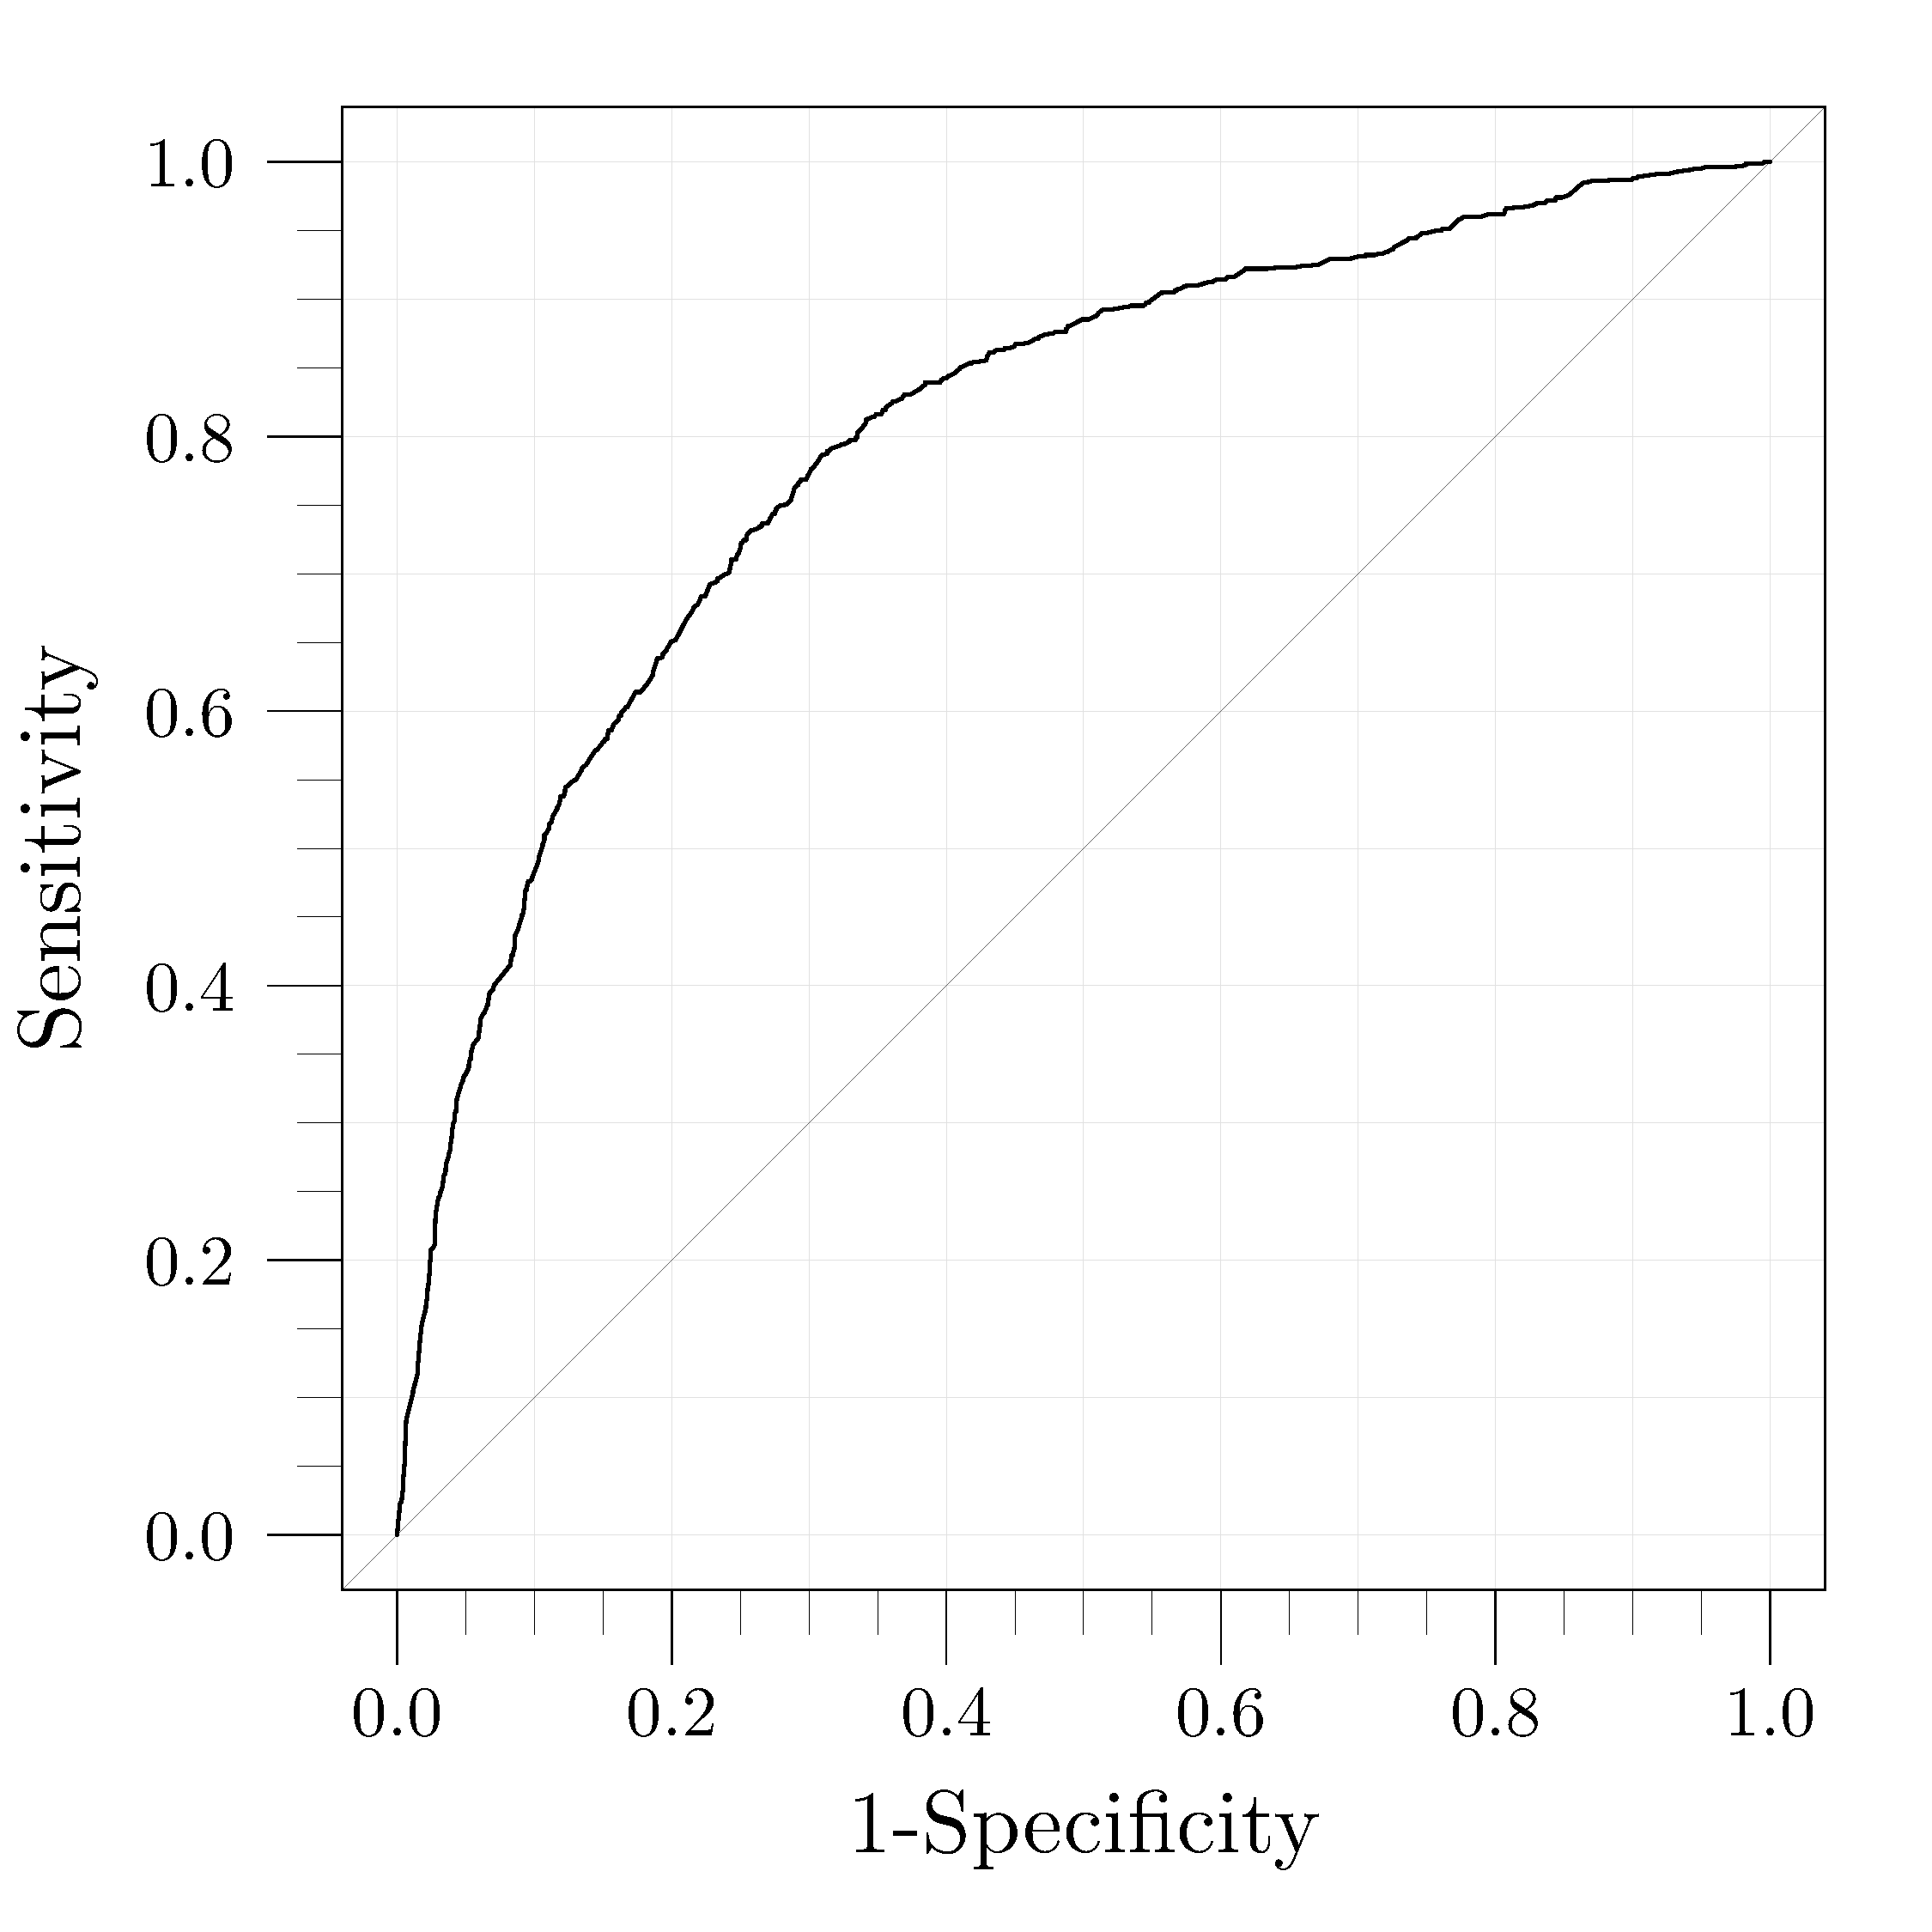
\includegraphics[width=9.5cm,height=9.5cm]{images/ROC_curve.pdf}
\caption[ROC curve of the selected GLM]{ROC curve of the logit model \texttt{fit10} ($\text{AUC}=0.801$). Maximum discrimination for values of sensitivity equal to 0.786 and specificity equal to 0.691.}
\label{fig:roc_curve}
\end{figure}

The logit link function facilitated further epidemiological inferences of the coefficients of the model, allowing for the interpretation of the explanatory variables in terms of odds ratio \cite{collet2003modelling}.
% With the model's parameters, and their respective standard errors, the odds of malaria infection occurrence to an individual can be obtained.
This is, comparing the odds of possible malaria infection when in relation to a similar individual that has a single variation in one of its variables.
%The standard error of the estimated of $\widehat{\beta}_1$ will be the standard error of the estimated log odds ratio, that is $\text{se}(\widehat{\beta}_1)=\text{se}(\log(e^{\beta_1}))$. With this results, an approximate 95\% confidence interval for the true odds ratio can be calculated by the expression XXX.\\
%The fact that this interval includes the unity suggests that the risk of infection occurring in persons XXX is not significantly different from those in the baseline level.
The analysis of the more significant transmission determinants and their respective odds ratios can create an association between the variations in malaria transmission intensity across the different situations that characterise the data.
%Investigating which are the significant risk factors that when combined cause a rise in prevalence of infection.
%Prevalence=probability of malaria infection occurre=the risk disease occurrence.\\
%Number of cases of the disease that occur given a period.\\
%The main purpose of estimating risks is to be able to make comparisons between the risk of disease at different levels of an risk factor, and thereby assess the association between the disease and that risk factor.\\
\newpage

\begin{table}[ht!]
\centering
\caption[Adjusted logistic GLM \texttt{fit10}]{Adjusted logistic GLM \texttt{fit10} with respective significant variables estimates, standard error and p-value. Odds ratio are given in relation to the indicator level of each transmission determinant (the odds ratios for these levels are equal to 1.00). For reference, the baseline level from the categorical demographical determinants are here indicated: $\textit{AgeGp}_{1-4}$, $\textit{Gender}_{Female}$, $\textit{EthGp}_{Other}$, and $\textit{Transect}_{WU3}$.}
\label{tab:fit11.glm}
\begin{adjustbox}{width=\linewidth}
% \begin{tabular}{ccrcrcc} 
% \toprule
% \multicolumn{1}{c}{Coefficient} & \multicolumn{1}{c}{\begin{tabular}[c]{@{}c@{}}Factor\\level\end{tabular}} & \multicolumn{1}{c}{\begin{tabular}[c]{@{}c@{}}Parameter\\estimate\end{tabular}} & \multicolumn{1}{c}{\begin{tabular}[c]{@{}c@{}}Standard\\error\end{tabular}} & \multicolumn{1}{c}{p-value} & \multicolumn{1}{c}{Odds ratio} & \multicolumn{1}{c}{\begin{tabular}[c]{@{}c@{}}95\% Confidence\\interval\end{tabular}}  \\ 
% \midrule
% (Intercept)                        & ---           & $-$0.775   & 0.212   & $<$0.001   & 0.46 & (0.30, 0.70)   \\
% \textit{Altitude}                  & ---           & $-$0.148   & 0.019   & $<$0.001   & 0.86 & (0.83, 0.89)   \\
% \textit{AgeGp}                     & 5$-$14        &  0.095     & 0.190   & 0.619      & 1.10 & (0.76, 1.60)   \\
%                                   & 15$-$45       & $-$1.712   & 0.196   & $<$0.001   & 0.18 & (0.12, 0.26)   \\
% \textit{EthGp}                     & Wachaga       &  0.623     & 0.320   & 0.052      & 1.86 & (1.00, 3.51)   \\
%                                   & Wapare        & $-$0.224   & 0.209   & 0.284      & 0.80 & (0.53, 1.21)   \\
%                                   & Wasambaa      &  0.192     & 0.160   & 0.231      & 1.21 & (0.89, 1.66)   \\
% \textit{Transect}                  & Rombo         & $-$0.971   & 0.322   & 0.003      & 0.38 & (0.20, 0.71)   \\
%                                   & N. Pare       & $-$1.478   & 0.337   & $<$0.001   & 0.23 & (0.12, 0.43)   \\
%                                   & S. Pare       & $-$0.420   & 0.247   & 0.089      & 0.66 & (0.40, 1.06)   \\
%                                   & W. Usamb. 1   &  0.463     & 0.214   & 0.030      & 1.59 & (1.04, 2.42)   \\
%                                   & W. Usamb. 2   &  0.014     & 0.212   & 0.946      & 1.01 & (0.67, 1.54)   \\
% \textit{AMA1}                      & 1             &  0.664     & 0.098   & $<$0.001   & 1.94 & (1.60, 2.36)   \\
% \textit{MSP1}                      & 1             &  0.500     & 0.097   & $<$0.001   & 1.65 & (1.36, 1.99)   \\
% \textit{MSP2}                      & 1             &  0.393     & 0.095   & $<$0.001   & 1.48 & (1.23, 1.79)   \\
% \textit{Altitude $\times$ AgeGp}   & 5$-$14        &  0.022     & 0.022   & 0.316      & 1.02 & (0.98, 1.07)   \\
%                                   & 15$-$45       &  0.114     & 0.023   & $<$0.001   & 1.12 & (1.07, 1.17)   \\
% \bottomrule
% \end{tabular}
\begin{tabular}{ccrcrcc} 
\toprule
\multicolumn{1}{c}{Coefficient} & \multicolumn{1}{c}{\begin{tabular}[c]{@{}c@{}}Factor\\level\end{tabular}} & \multicolumn{1}{c}{\begin{tabular}[c]{@{}c@{}}Parameter\\estimate, $\widehat{\beta}$\end{tabular}} & \multicolumn{1}{c}{\begin{tabular}[c]{@{}c@{}}Standard\\error\end{tabular}} & \multicolumn{1}{c}{p-value} & 
\multicolumn{1}{c}{\begin{tabular}[c]{@{}c@{}}Odds ratio,\\$e^{\widehat{\beta}}$\end{tabular}} &
\multicolumn{1}{c}{\begin{tabular}[c]{@{}c@{}}95\% Confidence\\interval\end{tabular}}  \\ 
\midrule
(Intercept)                        & ---           & $-$0.863   & 0.218   & $<$0.001   & 0.42   & (0.28, 0.65)   \\
\textit{Altitude}                  & ---           & $-$0.148   & 0.019   & $<$0.001   & 0.86   & (0.83, 0.89)   \\
\textit{AgeGp}                     & 5$-$14        &    0.112   & 0.190   & 0.555      & 1.12   & (0.77, 1.63)   \\
                                   & 15$-$45       & $-$1.681   & 0.197   & $<$0.001   & 0.19   & (0.13, 0.27)   \\
\textit{Gender}                    & Male          &    0.134   & 0.083   & 0.105      & 1.14   & (0.97, 1.34)   \\
\textit{EthGp}                     & Wachaga       &    0.619   & 0.320   & 0.053      & 1.86   & (1.00, 3.50)   \\
                                   & Wapare        & $-$0.228   & 0.209   & 0.276      & 0.80   & (0.53, 1.20)   \\
                                   & Wasambaa      &    0.194   & 0.160   & 0.226      & 1.21   & (0.89, 1.67)   \\
\textit{Transect}                  & Rombo         & $-$0.956   & 0.322   & 0.003      & 0.38   & (0.20, 0.72)   \\
                                   & N. Pare       & $-$1.470   & 0.337   & $<$0.001   & 0.23   & (0.12, 0.44)   \\
                                   & S. Pare       & $-$0.407   & 0.247   & 0.099      & 0.67   & (0.41, 1.08)   \\
                                   & W. Usamb. 1   &    0.472   & 0.214   & 0.027      & 1.60   & (1.05, 2.44)   \\
                                   & W. Usamb. 2   &    0.028   & 0.212   & 0.894      & 1.03   & (0.68, 1.56)   \\
\textit{AMA1}                      & 1             &    0.666   & 0.099   & $<$0.001   & 1.95   & (1.61, 2.36)   \\
\textit{MSP1}                      & 1             &    0.505   & 0.097   & $<$0.001   & 1.66   & (1.37, 2.00)   \\
\textit{MSP2}                      & 1             &    0.396   & 0.095   & $<$0.001   & 1.49   & (1.23, 1.79)   \\
\textit{Altitude $\times$ AgeGp}   & 5$-$14        &    0.022   & 0.022   & 0.335      & 1.02   & (0.98, 1.07)   \\
                                   & 15$-$45       &    0.114   & 0.023   & $<$0.001   & 1.12   & (1.07, 1.17)   \\
\bottomrule
\end{tabular}
\end{adjustbox}
\end{table}

In Mgome, 111 out of the 225 inhabitants were not infected.
Being the village with the highest prevalence of infection at the moment of sampling, one expected this selected baseline site to present good characteristics that, by comparison, could help to describe the different prevalence amongst all other villages.
% The logistic regression model shows that the risk of developing malaria infection during XXX was XXX times (p-value=XXX) higher in individuals XXX at the moment of sampling, than those who were XXX.
The odds ratio analysis suggested that the odds of an individual developing malaria infection at the reference village's altitude (0 meters, recall Section \ref{sec:4.1}) was significantly higher than those who inhabited any site with a higher altitude ($\widehat{\beta}=−0.148$ and $\text{p-value}<0.001$).
Being a proxy of malaria transmission, each 100 meters increased in altitude granted a reduction in odds of infection of approximately 14\% ($\widehat{OR}=0.86$).
This reduction showed how impactful altitude is, working as a protective factor.
The small confidence interval for the true odds ratio suggested a high precision of the odds of infection.
%This protective odds factor, proxy of malaria transmission intensity, has a small 95\% confidence interval.
% \textcolor{red}{FALAR AQUI DE COMO A VARIÁVEIS CLIMÁTICAS ESTÃO DIRECTAMENTE RELACIONADAS E REPRESENTADAS PELA ALTITUDE.}

% Agegp
Comparing the different age groups, only individuals older than 14 years old appeared to have their odds of infection significantly reduced ($\widehat{\beta}=-1.681$ and $\text{p-value}<0.001$).
This reduction -- $\widehat{OR}=0.19$, the biggest estimated in the categorical transmission determinants -- suggested older individuals were more prepared to live in sites of endemic transmission settings.
These older inhabitants, when in similar conditions as children from the reference level \textit{AgeGp}$_{1-4}$, would had their odds of being infected reduced by 73\% to 87\%.
There was no significant difference from infants to children with ages between 5 and 14 years old.
% The risk from individuals in the second age group ($\text{p-value}=0.619$) seems higher relatively to the first.
% However, with a confidence interval for the true odds ratio containing the unity, this level seems inconclusive, not influencing the prevalence of infection.
% The risk factor \textit{AgeGp}, with two degrees of freedom, estimates the odds ratio of its upper age groups relative to its indicator level.
% The risk of infection for individuals with ages comprehended in the second age group, $\textit{AgeGp}_{5-14}$ ($\text{p-value}=0.619$), shows a small increase of 6\% in prevalence.
% With its respective confidence interval for the true odds ratio ranging from 0.68 to 1.64, this level does not seem to significantly influence the prevalence of infection.
% However, individuals in the the third age group level, $\textit{AgeGp}_{15-45}$ ($\text{p-value}<0.001$), have their risk of infection reduced by 74\% to 88\%, when compared to the reference age group.
% This reduction (the biggest estimated in the categorical risk factors) suggests that individuals older than 14 years old are usually protected enough, and when in similar conditions as children from the first age group, their risk of being infected would be 82 times smaller.
% Gender
The binary risk factor \textit{Gender}, was kept throughout the model's construction.
Ultimately it did not seem to play a significant role influencing prevalence of infection ($\widehat{\beta}=0.134$ and $\text{p-value}=0.105$).

% Ethnic
Assessing the different ethnicities, only the Wachaga ethnic group ($\widehat{\beta}=0.619$ and $\text{p-value}=0.053$) seemed to produce a borderline significant result on the response variable, with $\widehat{OR}=1.86$.
Despite the inclusion of the unity in the estimated confidence interval for the true odds ratio, this level suggested a tendency.
In similar conditions, individuals from this ethnic group would had higher odds infection than someone from the ethnicities found in Mgome, $\textit{EthGp}_{Other}$, at the moment of sampling.
% Maybe by omitting data from some individuals in the analysis could adjust the estimated odds ratio to some extend, and removing the unity from the confidence interval, resulting in some more informative results.
The odds of infection in individuals from the remaining ethnic groups Wapare ($\widehat{\beta}=-0.228$ and $\text{p-value}=0.276$) and Wasambaa ($\widehat{\beta}=0.194$ and $\text{p-value}=0.226$) did not appear significantly different in the analysis.
% , suggest individuals in these ethnic groups have a increased risk of being infected than someone with Other ethnicity, under the same conditions.
% As for the Wapare ethnic group ($\text{p-value}=0.284,\ \text{OR}=0.80$), the relative risk of an individual from this ethnic group being infected is reduced.
% Even though different ethnicities granted different levels of risk of malaria prevalence, the exclusion of data from some individuals in the analysis could adjust the estimated odds ratio to some extend, resulting in some more informative or precise confidence intervals. OUT

% Transect
The covariate \textit{Transect} showed how malaria transmission intensity varied between the two Tanzanian regions, across the different defined transects.
If compared in the same conditions, individuals from the four villages in Rombo ($\widehat{\beta}=-0.956$ and $\text{p-value}=0.003$) had their odds of being infected reduced by 62\% ($\widehat{OR}=0.38$), while villages in the North Pare ($\widehat{\beta}=-1.470$ and $\text{p-value}<0.001$) had their odds reduced by 77\% ($\widehat{OR}=0.23$).
The latter showed the more significant and precise odds reduction.
Similar to the tendency value in $\textit{EthGp}_{Wachaga}$, with the inclusion of the unity within the confidence interval of the true odds ratio, villages belonging to South Pare seem to present reduced odds for malaria infection.
%However, since the confidence interval for the true odds ratio includes the unity, the results fom South Pare can be somewhat inconclusive.
In the Tanga region, West Usambara 1 ($\widehat{\beta}=0.472$ and $\text{p-value}=0.027$) suggested a higher odds of infection relatively to Mgome, having prevalence growing by 1.60 times.
West Usambara 2 ($\widehat{\beta}=0.028$ and $\text{p-value}=0.894$) did not seem to significantly impact prevalence.
% The analysis of the confidence intervals for the true odds ratio in the different transects marked \textit{Transect} as a highly determinant factor for malaria infection.

% AMA1 MSP1 MSP2
The presence of each one of exposure antigens, \textit{AMA1}, \textit{MSP1}, or \textit{MSP2} ($\widehat{\beta}=0.666$, $\widehat{\beta}=0.505$, and, $\widehat{\beta}=0.022$, respectively, all with $\text{p-values}<0.001$), when compared to their respective control level, consistently increased the prevalence as a consequence for exposure ($\widehat{OR}_{AMA1}=1.95$, $\widehat{OR}_{MSP1}=1.66$, $\widehat{OR}_{MSP2}=1.49$, respectively).
This increment suggested how impactful the antigens can be.
Since in normal conditions any non exposed individual is expected to not develop specific antimalarial antibodies, thus not being at risk of becoming infected, the simple detection of an antigen by itself implies a increase on the odds of infection due to exposure.
Depending on the three antigens, odds of infection increased from almost 50\%, when MSP2 was detected, to almost doubling the odds whenever antigen AMA1 was detected in the serum.
%(0.000, 1.02)This interval barely includes the unity, suggesting that the evidence that XXX protects against malaria infection is now significant at about the 5\% level. Omitting the data from some individuals from the analysis could decrease the estimated odds ratio to some extend, resulting in a more informative result.


%%%%%%%%%%%
% SUMMARY %
%%%%%%%%%%%
\section{Summary}

% Primeira frase é conversa fiada...
The identification and study of the primary malaria infection covariates in a region is an approach that can be made as soon as enough variables are collected.
These analyses present some flexibility, as different and more specific transmission determinants can be included for consideration, depending on the study objectives \cite{binka1995risk}.
When overseeing the regions of the Northeast Tanzania, the best combination of transmission determinants through the GLMs helped making inferences about the relative proportion of infected malaria cases across the different sites at the time of sampling.
Also, through the regression coefficient estimates and estimated odds ratio, the relative transmission intensity across the different villages was compared, inferring about impactful determinants that could originate the prevalence estimated and transmission intensity heterogeneity measured.
% In distant or contrasting regions, the identification of the important determinants can potentially lead to hotspots for prevalence of infection.

The application of different categorical variables onto the logistic regression model \texttt{fit10} identified the more susceptible levels to infection.
In the demographical determinants, both \textit{AgeGp} and \textit{Transect} proved to be important categorical risk factors to describe occurrence of infection.
% As the latter can influence the prevalence of infection, the effect of \textit{AgeGp} also reflects the acquired immunity to parasites.
The odds of adults becoming infected with malaria is lower since they might have developed specific immunity throughout periods of recurrent exposure and reinfections.
The impact of these transmission determinants can be related to the geographical conditions of each site, modelling the environment and overall anthropomorphic characteristic of its inhabitants.
Variable \textit{Altitude} also played an important role.
As a proxy for transmission intensity, a value increment in this continuous risk factor can be interpreted as a decrease in temperature and humidity, gradually reducing the number of \textit{Anopheles} mosquitoes, \textit{P. falciparum} transmitters.

Binary variables for the antigen responses presented elevated odds for malaria infection.
All three exposure antigens worked well as stable predictors for malaria exposure, being indirectly influenced by the demographical determinants delineating the level of exposure, and presenting a direct effect in the immunological uplift (aquired immunity) over time gained by an individual \cite{shelton2015genetic}.
With the antigens identified as good indicators for exposure to malaria parasites and overall transmission intensity, when measured at different ages, Chapter \ref{ch:5.0} focused the detection of the immunologic responses as outcome of interest.
Specific stochastic models were applied, measuring transmission intensity produced by different characteristics from each village, across the sequence of different ages.
% Is the model good?\\
% What's missing?\\
% Disadvantages of using this model.
%The basis for choosing a single model from amongst them will not then rest on statistical grounds alone.
%while in areas of lower transmission many cases also occur in older children and adults.
% OR can also have some limitations, as odds ratios below 1 are more difficult to interpret than those above it. This is perhaps due to the fact that from below, odds ratios are limited by 0, whereas from above, there is no limit.
% Referir artigo \cite{shelton2015genetic} que fala dos Ab MSP1, MSP2, e AMA1 nas várias regiões, e como eles evoluem ao longo das faixas etárias.
